\documentclass[conference]{IEEEtran}

\usepackage{amsmath,amssymb,amsfonts}
\usepackage{bm}
\usepackage{cite}
\usepackage{graphicx}
\usepackage{booktabs}
\usepackage{array}
\usepackage{amsthm}
\usepackage{url}
\usepackage{xcolor}
\usepackage{tikz}
\usetikzlibrary{arrows.meta,positioning,calc,decorations.pathreplacing}

\newtheorem{proposition}{Proposition}
\newtheorem{definition}{Definition}
\newtheorem{remark}{Remark}

\newcommand{\C}{\mathbb{C}}
\newcommand{\Real}{\operatorname{Re}}
\newcommand{\Imag}{\operatorname{Im}}
\newcommand{\spec}{\operatorname{spec}}
\newcommand{\norm}[1]{\left\lVert #1 \right\rVert}
\newcommand{\dd}{\mathrm{d}}

\title{Weak Nodes and Weak Links Are Not Graph-Centrality Objects in IBR Grids}

\author{
\IEEEauthorblockN{Jorge L. Mayorga Taborda}
\IEEEauthorblockA{Universidad de los Andes, Bogota, Colombia\\
Email: author@example.com}
}

\begin{document}
\maketitle

\begin{abstract}
Weak nodes and weak links in inverter-based-resource (IBR) grids are often discussed as if they were graph objects: highly central buses, heavily loaded branches, low short-circuit-strength locations, or large entries of a Laplacian eigenvector. This paper argues that this is the wrong object for damping-margin weakness once inverter and controller states participate in the critical mode. The reduced object is a controller-aware nonlinear eigenvalue problem (NEP), obtained by Schur-complement condensation of controller states. In this representation, a line or node is weak only relative to an action, a pole family, and the frequency-dependent controller self-energy. We formalize this statement with a local NEP sensitivity certificate and show that a graph-only centrality score cannot determine the sign of a damping-margin change when condensed controller poles are present. The same framework separates ordinary damping-ratio geometry from a stricter \emph{control-resonant Braess} mechanism: strengthening a line may reduce damping because it moves a network-family mode toward a PLL-dominated controller pole. On IEEE 39-bus ANDES cases, a Beyn contour solver for the Schur NEP reproduces the full ANDES critical poles to numerical precision, including a 13.742 Hz PLL-family Mix60 mode missed by scalar reductions. A registered line audit over 460 perturbations finds 40 strict resonant records; the clearest case is Line 20--34 in Mix60/no-PSS, where the self-energy term predicts the network-mode damping decrease with 0.2\% relative error. The contribution is not a new graph centrality, but a dynamic certificate explaining when graph centrality is the wrong language.
\end{abstract}

\begin{IEEEkeywords}
Inverter-based resources, damping margin, weak nodes, weak links, Braess paradox, nonlinear eigenvalue problem, Schur complement, phase-locked loop.
\end{IEEEkeywords}

\section{Introduction}

Power-grid planning often uses graph language. A weak bus is associated with electrical distance, short-circuit strength, modal participation, or centrality; a weak line is associated with loading, cut structure, or Laplacian sensitivity. These ideas remain useful for static network questions, but they can become misleading for damping-margin questions in inverter-dominated grids. The reason is simple: in detailed IBR models, the damping observed in the least-damped pole may be supplied by PLL, exciter, stabilizer, governor, grid-following, or grid-forming controller states rather than by a static nodal damping coefficient.

This paper develops a narrow alternative. A weak element is not defined by where it sits in the graph. It is defined by how a physically admissible action moves the damping-margin pole of the controller-aware reduced eigenproblem. To keep the object transparent, we derive the certificate from the electrical power-flow equations before introducing the Schur reduction. The result is a local certificate:
\[
  \begin{split}
  \text{weak element}={}&
  \text{negative pole-margin sensitivity}\\
  &+\text{control-resonance exposure}.
  \end{split}
\]
This viewpoint is especially important for Braess-like claims. If a line reinforcement raises oscillation frequency while the decay rate does not increase enough, the damping ratio can fall. That is a geometric damping-ratio effect, not necessarily a network paradox. A stricter and more IBR-specific mechanism appears when reinforcement moves a network-family mode toward a nearby controller pole, so the frequency-dependent self-energy of the controller dominates the damping loss. We call this a control-resonant Braess mechanism.

The paper makes three contributions.
\begin{enumerate}
\item It defines controller-aware weak-node and weak-link certificates from Schur-NEP pole sensitivities rather than graph centrality.
\item It proves a non-identifiability result: graph-only centrality cannot determine weak elements when the controller self-energy is active, because the graph can be fixed while the sign of the damping sensitivity changes through condensed controller poles.
\item It gives a minimal three-bus witness and validates the mechanism on IEEE 39-bus ANDES artifacts: the Schur NEP reproduces full ANDES critical poles, and a line audit finds strict resonant reinforcement reversals under a PLL-dominated self-energy term.
\end{enumerate}
The scope is deliberately limited. We do not claim that all line-reinforcement reversals are resonant, that graph centrality is useless for static planning, or that the proposed certificate is already a full planning optimizer. The result is a mechanism paper: it identifies the dynamic object that graph centrality misses. Figs.~\ref{fig:failure_modes}--\ref{fig:certificate_workflow} also include the associated inertia warning from the project gates: adding inertia can reduce damping in GENROU/reduced-model tests, but GFM virtual-inertia assignment over the controller-aware bridge remains a separate validation task.

\begin{figure*}[t]
\centering
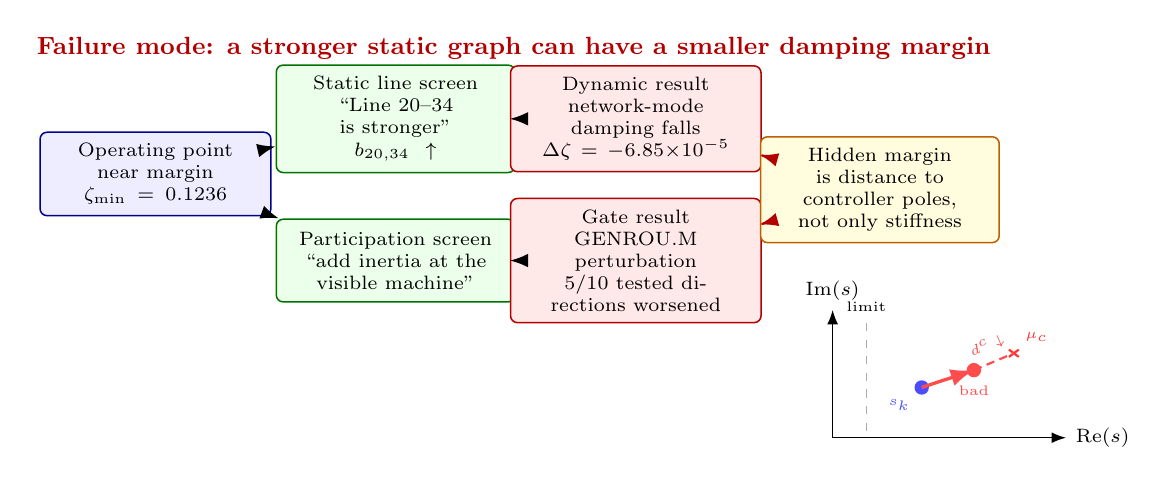
\begin{tikzpicture}[
  font=\scriptsize,
  >=Latex,
  box/.style={draw, rounded corners=2.5pt, align=center, inner sep=4pt, line width=0.55pt, minimum height=1.05cm},
  base/.style={box, fill=blue!7, draw=blue!55!black, text width=2.65cm},
  naive/.style={box, fill=green!8, draw=green!45!black, text width=2.75cm},
  warn/.style={box, fill=red!9, draw=red!70!black, text width=2.9cm},
  note/.style={box, fill=yellow!13, draw=orange!75!black, text width=2.75cm}
]
\node[font=\small\bfseries, red!70!black] at (6.1,5.15)
  {Failure mode: a stronger static graph can have a smaller damping margin};

\node[base] (base) at (1.55,3.55)
  {Operating point\\near margin\\$\zeta_{\min}=0.1236$};
\node[naive] (linegreen) at (4.6,4.25)
  {Static line screen\\``Line 20--34 is stronger''\\$b_{20,34}\uparrow$};
\node[warn] (linebad) at (7.65,4.25)
  {Dynamic result\\network-mode damping falls\\$\Delta\zeta=-6.85{\times}10^{-5}$};
\node[naive] (inertiagreen) at (4.6,2.45)
  {Participation screen\\``add inertia at the visible machine''};
\node[warn] (inertiabad) at (7.65,2.45)
  {Gate result\\GENROU.M perturbation\\5/10 tested directions worsened};
\node[note] (hidden) at (10.75,3.35)
  {Hidden margin\\is distance to\\controller poles,\\not only stiffness};

\draw[->, thick] (base) -- (linegreen);
\draw[->, thick] (linegreen) -- (linebad);
\draw[->, thick] (base) -- (inertiagreen);
\draw[->, thick] (inertiagreen) -- (inertiabad);
\draw[->, thick, red!70!black] (linebad) -- (hidden);
\draw[->, thick, red!70!black] (inertiabad) -- (hidden);

\begin{scope}[shift={(10.15,0.20)}, x=0.78cm, y=0.58cm]
  \draw[->, line width=0.5pt] (0,0) -- (3.8,0) node[right, font=\scriptsize] {$\Real(s)$};
  \draw[->, line width=0.5pt] (0,0) -- (0,2.8) node[above, font=\scriptsize] {$\Imag(s)$};
  \draw[dashed, gray!65] (0.55,0.15) -- (0.55,2.55) node[above, font=\tiny, black] {limit};
  \coordinate (s0) at (1.45,1.1);
  \coordinate (sbad) at (2.30,1.48);
  \coordinate (mu) at (2.95,1.85);
  \fill[blue!70] (s0) circle (2.6pt) node[below left=1pt, font=\tiny] {$s_k$};
  \fill[red!70] (sbad) circle (2.6pt);
  \draw[->, red!70, very thick] (s0) -- (sbad);
  \draw[red!80, line width=0.8pt] (mu) +(-0.08,-0.08) -- +(0.08,0.08);
  \draw[red!80, line width=0.8pt] (mu) +(-0.08,0.08) -- +(0.08,-0.08);
  \node[red!80, above right=1pt of mu, font=\tiny] {$\mu_c$};
  \draw[densely dashed, red!70, thick] (sbad) -- node[above, sloped, font=\tiny] {$d^c\downarrow$} (mu);
  \node[red!70, below=2pt of sbad, font=\tiny] {bad};
\end{scope}
\end{tikzpicture}
\caption{Why Fig.~\ref{fig:certificate_workflow} is needed. Static planning signals can point in the wrong direction for damping: a line reinforcement may increase synchronizing stiffness while reducing the damping ratio, and an inertia perturbation can worsen damping in the validated GENROU gate. The common failure is that neither static graph strength nor modal visibility measures distance to condensed controller poles.}
\label{fig:failure_modes}
\end{figure*}

\begin{figure*}[t]
\centering
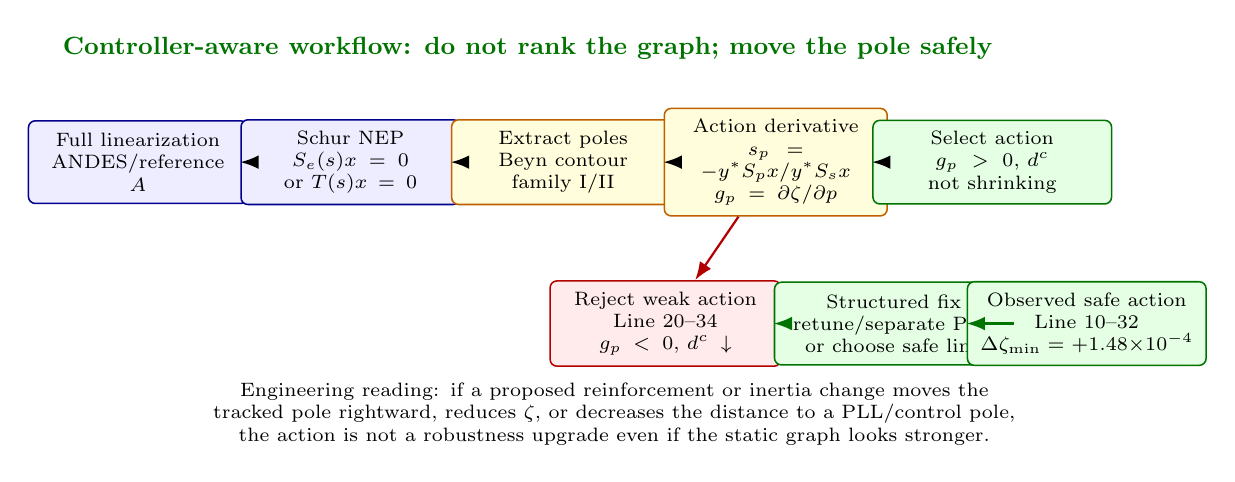
\begin{tikzpicture}[
  font=\scriptsize,
  >=Latex,
  box/.style={draw, rounded corners=2.5pt, align=center, inner sep=4pt, line width=0.55pt, minimum height=1.05cm},
  data/.style={box, fill=blue!7, draw=blue!55!black, text width=2.5cm},
  calc/.style={box, fill=yellow!14, draw=orange!75!black, text width=2.55cm},
  decision/.style={box, fill=green!10, draw=green!45!black, text width=2.75cm},
  stop/.style={box, fill=red!8, draw=red!70!black, text width=2.65cm}
]
\node[font=\small\bfseries, green!45!black] at (6.05,4.7)
  {Controller-aware workflow: do not rank the graph; move the pole safely};
\node[data] (full) at (1.1,3.25)
  {Full linearization\\ANDES/reference\\$A$};
\node[data] (schur) at (3.8,3.25)
  {Schur NEP\\$S_e(s)x=0$\\or $T(s)x=0$};
\node[calc] (poles) at (6.5,3.25)
  {Extract poles\\Beyn contour\\family I/II};
\node[calc] (sens) at (9.2,3.25)
  {Action derivative\\$s_p=-y^\ast S_px/y^\ast S_sx$\\$g_p=\partial\zeta/\partial p$};
\node[decision] (safe) at (11.95,3.25)
  {Select action\\$g_p>0$, $d^c$ not shrinking};

\node[stop] (reject) at (7.8,1.20)
  {Reject weak action\\Line 20--34\\$g_p<0$, $d^c\downarrow$};
\node[decision] (fix) at (10.7,1.20)
  {Structured fix\\retune/separate PLL\\or choose safe link};
\node[decision] (margin) at (13.15,1.20)
  {Observed safe action\\Line 10--32\\$\Delta\zeta_{\min}=+1.48{\times}10^{-4}$};

\draw[->, thick] (full) -- (schur);
\draw[->, thick] (schur) -- (poles);
\draw[->, thick] (poles) -- (sens);
\draw[->, thick] (sens) -- (safe);
\draw[->, thick, red!70!black] (sens) -- (reject);
\draw[->, thick, green!45!black] (reject) -- (fix);
\draw[->, thick, green!45!black] (fix) -- (margin);
\node[align=center, text width=12.0cm] at (7.15,0.05)
{Engineering reading: if a proposed reinforcement or inertia change moves the
tracked pole rightward, reduces $\zeta$, or decreases the distance to a
PLL/control pole, the action is not a robustness upgrade even if the static graph
looks stronger.};
\end{tikzpicture}
\caption{Controller-aware robustness workflow. The certificate turns weak-node
and weak-link analysis into a typed engineering statement: the element is weak
for a specified mode, action, and controller configuration.}
\label{fig:certificate_workflow}
\end{figure*}

\section{From Electrical Model to Damping Certificate}

This section derives the object used in the paper from the standard small-signal
power-system equations. The purpose is not to introduce a new network model, but
to show exactly where the usual graph object stops being sufficient.

\begin{figure*}[t]
\centering
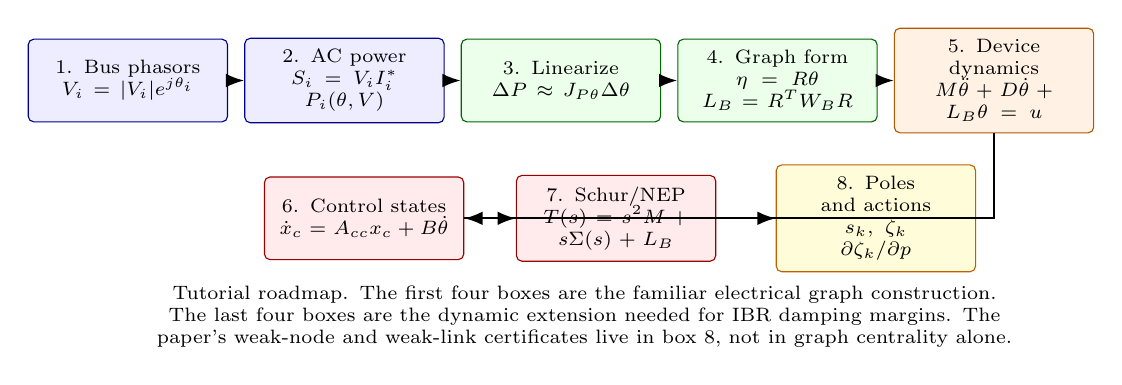
\begin{tikzpicture}[
  font=\scriptsize,
  >=Latex,
  stepbox/.style={draw, rounded corners=2pt, align=center, inner sep=4pt, minimum height=1.05cm, text width=2.25cm},
  phys/.style={stepbox, fill=blue!7, draw=blue!55!black},
  graph/.style={stepbox, fill=green!8, draw=green!40!black},
  dyn/.style={stepbox, fill=orange!10, draw=orange!70!black},
  ctrl/.style={stepbox, fill=red!8, draw=red!60!black},
  cert/.style={stepbox, fill=yellow!15, draw=orange!75!black},
  arr/.style={->, thick}
]
\node[phys] (p1) at (0,0) {1. Bus phasors\\$V_i=|V_i|e^{j\theta_i}$};
\node[phys] (p2) at (2.75,0) {2. AC power\\$S_i=V_iI_i^\ast$\\$P_i(\theta,V)$};
\node[graph] (p3) at (5.5,0) {3. Linearize\\$\Delta P\approx J_{P\theta}\Delta\theta$};
\node[graph] (p4) at (8.25,0) {4. Graph form\\$\eta=R\theta$\\$L_B=R^TW_BR$};
\node[dyn] (p5) at (11.0,0) {5. Device dynamics\\$M\ddot\theta+D\dot\theta+L_B\theta=u$};
\node[ctrl] (p6) at (3.0,-1.75) {6. Control states\\$\dot x_c=A_{cc}x_c+B\dot\theta$};
\node[ctrl] (p7) at (6.2,-1.75) {7. Schur/NEP\\$T(s)=s^2M+s\Sigma(s)+L_B$};
\node[cert] (p8) at (9.5,-1.75) {8. Poles and actions\\$s_k,\ \zeta_k$\\$\partial\zeta_k/\partial p$};
\draw[arr] (p1) -- (p2);
\draw[arr] (p2) -- (p3);
\draw[arr] (p3) -- (p4);
\draw[arr] (p4) -- (p5);
\draw[arr] (p5.south) |- (p6.east);
\draw[arr] (p6) -- (p7);
\draw[arr] (p7) -- (p8);
\node[align=center, font=\scriptsize, text width=11.5cm] at (5.8,-3.0)
{Tutorial roadmap. The first four boxes are the familiar electrical graph construction.
The last four boxes are the dynamic extension needed for IBR damping margins. The
paper's weak-node and weak-link certificates live in box 8, not in graph centrality alone.};
\end{tikzpicture}
\caption{Step-by-step route from phasors to the controller-aware damping certificate.}
\label{fig:tutorial_pipeline}
\end{figure*}

\subsection{Electrical Network and Linearized Power Flow}

\noindent\textbf{Step 1: represent each bus by a phasor.}
At a bus $i$, the balanced positive-sequence voltage is represented by the
phasor
\begin{equation}
  V_i = |V_i|e^{j\theta_i},
  \label{eq:phasor}
\end{equation}
where $|V_i|$ is the voltage magnitude and $\theta_i$ is the phase angle with
respect to the synchronous reference. The time waveform is recovered as
$v_i(t)=\sqrt{2}\Real\{V_i e^{j\omega_0t}\}$. This phasor representation is
important because electromechanical oscillations and PLL dynamics are primarily
angle/frequency phenomena: the small variables are not the absolute voltages,
but the angle deviations $\Delta\theta_i$ and frequency deviations
$\Delta\omega_i=\Delta\dot\theta_i$.

\noindent\textbf{Step 2: write nodal current and complex power.}
Let $Y=G+jB$ be the network admittance matrix. The complex current injection is
$I=YV$, i.e.,
\begin{equation}
  I_i=\sum_{j=1}^{n}Y_{ij}V_j .
  \label{eq:current}
\end{equation}
The complex power injection at bus $i$ is
\begin{equation}
  S_i=P_i+jQ_i=V_i I_i^\ast .
  \label{eq:complexpower}
\end{equation}
Expanding the active-power component gives
\begin{equation}
  P_i=\sum_{j=1}^{n}|V_i||V_j|
  \left[
  G_{ij}\cos(\theta_i-\theta_j)
  +B_{ij}\sin(\theta_i-\theta_j)
  \right].
  \label{eq:acpower}
\end{equation}
This is the nonlinear AC network equation. The dynamic model below uses its
Jacobian at the operating point.

\noindent\textbf{Step 3: linearize active power with respect to angles.}
For high-voltage transmission lines, conductance is small compared with
susceptance, so the active-power sensitivity to angle is dominated by the
susceptive term. Linearizing \eqref{eq:acpower} around an operating point
$\theta^0$ gives, for a line $(i,j)$,
\begin{equation}
  \Delta P_{ij}=b_{ij}(\Delta\theta_i-\Delta\theta_j),
  \qquad
  b_{ij}=|V_i||V_j|B_{ij}\cos(\theta_i^0-\theta_j^0).
  \label{eq:lineflow}
\end{equation}
Thus every line measures an angle difference. This is the physical reason a
graph Laplacian appears.
Equivalently, the active-power Jacobian has the local entries
\begin{equation}
  \frac{\partial P_i}{\partial\theta_j}\bigg|_{\theta^0}
  =
  \begin{cases}
  -b_{ij}, & i\neq j,\\
  \sum_{\ell\neq i}b_{i\ell}, & i=j,
  \end{cases}
  \label{eq:jacentries}
\end{equation}
up to the chosen sign convention for injection versus imbalance.

\noindent\textbf{Step 4: stack line differences with an incidence matrix.}
To make the graph construction explicit, orient the $m$ lines arbitrarily and
let $R\in\mathbb{R}^{m\times n}$ be the incidence matrix,
\begin{equation}
  R_{\ell i}=1,\quad R_{\ell j}=-1
  \quad\text{for line }\ell=(i,j).
  \label{eq:incidence}
\end{equation}
Then the vector of line angle drops is
\begin{equation}
  \eta = R\theta,
  \label{eq:edgegradient}
\end{equation}
and the vector of linearized line-power flows is
\begin{equation}
  f = W_B R\theta,
  \qquad
  W_B=\operatorname{diag}(b_\ell).
  \label{eq:edgeflow}
\end{equation}
Nodal active-power imbalance is the signed sum of incident line flows:
\begin{equation}
  \Delta P_e=R^T f
  =R^TW_BR\,\Delta\theta
  =L_B\Delta\theta.
  \label{eq:lapflow}
\end{equation}
Therefore
\begin{equation}
  L_B=R^TW_BR,
  \label{eq:lapincidence}
\end{equation}
or, entrywise,
\begin{equation}
  (L_B)_{ij}=
  \begin{cases}
    \sum_{\ell\neq i}b_{i\ell}, & i=j,\\
    -b_{ij}, & i\neq j\ \text{and line }(i,j)\text{ exists},\\
    0, & \text{otherwise}.
  \end{cases}
  \label{eq:lapentries}
\end{equation}
The graph is therefore not an abstract analogy: it is the matrix form of
linearized active-power balance. The nodes are bus phasor angles, the edges are
line susceptance-weighted angle differences, and the Laplacian maps angle
deviations into electrical power imbalance.

This is also the point where a graph-only analysis usually enters. A line
reinforcement increases one weight $b_\ell$ in $W_B$, hence increases a positive
semidefinite rank-one term
\begin{equation}
  \Delta L_B = \Delta b_\ell\, r_\ell^T r_\ell,
  \label{eq:line_rankone}
\end{equation}
where $r_\ell$ is the incidence row of the line. If only \eqref{eq:lapflow} is
inspected, a larger $b_\ell$ looks like a stronger synchronizing network. The
rest of the paper shows why this conclusion can be incomplete for damping.

\subsection{Swing and Grid-Forming Interface Dynamics}

\noindent\textbf{Step 5: connect electrical imbalance to device motion.}
For a synchronous generator, or a grid-forming inverter represented by a virtual
swing equation, the retained electromechanical variables satisfy
\begin{align}
  \dot\theta_i &= \omega_i, \label{eq:thetadot}\\
  M_i\dot\omega_i &=
  - (L_B\theta)_i - D_i\omega_i + u_i,
  \label{eq:swing}
\end{align}
where $M_i$ is physical or virtual inertia, $D_i$ is local damping or droop, and
$u_i$ collects controller and auxiliary feedback channels not yet modeled. This
is the small-signal power-balance law: inertial power equals mechanical/control
injection minus electrical imbalance minus damping.
In vector form,
\begin{equation}
  M\ddot\theta+D\dot\theta+L_B\theta=u.
  \label{eq:secondorderbasic}
\end{equation}
If $u=0$, this is a quadratic dynamical system. Introduce
$\omega=\dot\theta$ and $x_{\mathrm{em}}=[\theta^T,\omega^T]^T$. The
corresponding first-order state matrix is
\begin{align}
  \frac{d}{dt}
  \begin{bmatrix}\theta\\\omega\end{bmatrix}
  &=
  A_{\mathrm{em}}
  \begin{bmatrix}\theta\\\omega\end{bmatrix},
  \label{eq:em_state}\\
  A_{\mathrm{em}}
  &=
  \begin{bmatrix}
  0&I\\
  -M^{-1}L_B&-M^{-1}D
  \end{bmatrix}.
  \label{eq:aem_def}
\end{align}
The poles of the retained electromechanical model are the eigenvalues of
$A_{\mathrm{em}}$, equivalently the roots of the quadratic eigenvalue problem
\begin{equation}
  \det(s^2M+sD+L_B)=0.
  \label{eq:qep_basic}
\end{equation}
If $D$ is proportional to $M$, the modes decouple in the eigenvectors of the
mass-normalized Laplacian $M^{-1/2}L_BM^{-1/2}$. With
$q_k^\ast M q_\ell=\delta_{k\ell}$ and $q_k^\ast L_B q_k=\nu_k$, the modal
damping ratio is
\begin{equation}
  \zeta_k=\frac{\delta_k}{2\sqrt{\nu_k}},
  \qquad
  \delta_k=q_k^\ast D q_k.
  \label{eq:modalzeta}
\end{equation}
This scalar formula is useful, but it already shows a warning: increasing
stiffness $\nu_k$ does not automatically increase damping ratio unless the
modal damping $\delta_k$ increases enough.

\subsection{Controller States and the Hidden Channel}

\noindent\textbf{Step 6: add the controller states that the graph does not see.}
IBR models add states that are not present in \eqref{eq:secondorderbasic}:
PLL filters, current-control states, outer-loop states, virtual-oscillator
states, power controllers, exciters, stabilizers, governors, and measurement
filters. Let $x_c$ denote those states and suppose that, after linearization,
they interact with the retained network variables as
\begin{align}
  M\ddot\theta+D_0\dot\theta+L_B\theta+Kx_c&=0,
  \label{eq:networkcontrol}\\
  \dot x_c&=A_{cc}x_c+B\dot\theta .
  \label{eq:controlstates}
\end{align}
\noindent\textbf{Step 7: eliminate the controller states in the Laplace domain.}
Taking Laplace transforms of \eqref{eq:networkcontrol}--\eqref{eq:controlstates}
gives
\begin{align}
  (s^2M+sD_0+L_B)\theta(s)+Kx_c(s)&=0,
  \label{eq:lap_network}\\
  (sI-A_{cc})x_c(s)&=sB\theta(s).
  \label{eq:lap_control}
\end{align}
For $s\notin\spec(A_{cc})$,
\begin{equation}
  x_c(s)=s(sI-A_{cc})^{-1}B\theta(s).
  \label{eq:xc_elim}
\end{equation}
Substituting \eqref{eq:xc_elim} into \eqref{eq:lap_network} gives
\begin{equation}
  \left[
  s^2M+s\left(D_0+K(sI-A_{cc})^{-1}B\right)+L_B
  \right]\theta(s)=0 .
  \label{eq:derivednep}
\end{equation}
The bracketed matrix is a nonlinear eigenvalue problem (NEP). The term
\begin{equation}
  \Sigma(s)=D_0+K(sI-A_{cc})^{-1}B
  \label{eq:sigmadef_intro}
\end{equation}
is the controller self-energy. It is frequency dependent and has poles at
$\spec(A_{cc})$. Therefore the margin is not determined only by the graph
stiffness $L_B$ or by a constant damping matrix. A line, inertia, or controller
change is dangerous when it moves a relevant zero of \eqref{eq:derivednep}
toward a low-damped controller pole or rotates the mode into a poorly damped
controller channel.

\subsection{Why Poles, Not Only Eigenvectors, Define Stability Margin}

\noindent\textbf{Step 8: define stability from poles.}
For any linearized model, a mode has the time dependence $e^{st}v$. If
$s=\sigma+j\omega$, then $\sigma$ gives the exponential decay rate and
$|\omega|/(2\pi)$ gives the oscillation frequency. The mode is stable only when
$\sigma<0$. Its damping ratio is
\begin{equation}
  \zeta(s)=-\frac{\sigma}{\sqrt{\sigma^2+\omega^2}}.
  \label{eq:pole_zeta_intro}
\end{equation}
The damping margin is the minimum $\zeta(s)$ over the relevant oscillatory
poles. This is why a weak element cannot be defined by an eigenvector entry
alone. An eigenvector says where a mode is visible; the pole says whether the
mode decays, how fast it decays, and how close it is to a controller resonance.

In the scalar graph model, strengthening a line changes only $L_B$ and therefore
changes modal stiffness. In the controller-aware model, the same action changes
the zero of \eqref{eq:derivednep} through both $L_B$ and the resolvent
$(sI-A_{cc})^{-1}$. When $s$ is close to a controller pole $\mu\in\spec(A_{cc})$,
small physical changes can produce large pole motion because the denominator
$s-\mu$ is small. This is the hidden-margin mechanism: the operating point can
look acceptable in a graph or frequency-only screen while the damping pole is
already close to a control resonance.

\begin{figure*}[t]
\centering
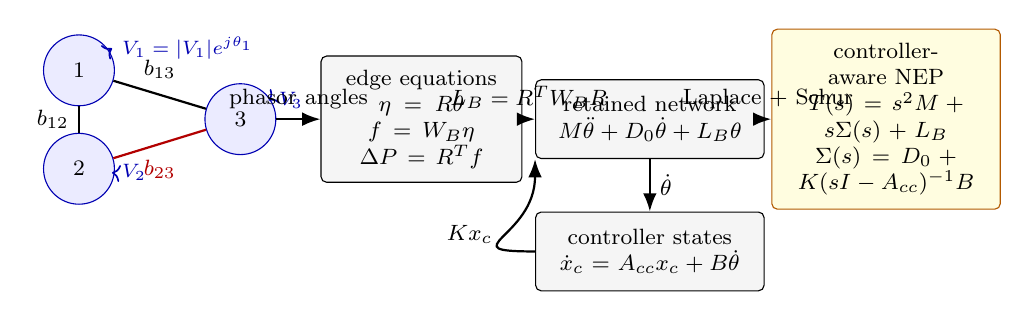
\begin{tikzpicture}[
  font=\footnotesize,
  bus/.style={circle, draw=blue!70!black, fill=blue!8, minimum size=9mm, inner sep=0pt},
  ph/.style={->, blue!70!black, line width=0.6pt},
  block/.style={draw, rounded corners=2pt, align=center, fill=gray!8, inner sep=5pt, minimum height=1.0cm},
  arr/.style={->, thick, >=Latex}
]
\node[bus] (b1) at (0,1.25) {1};
\node[bus] (b2) at (0,0) {2};
\node[bus] (b3) at (2.05,0.63) {3};
\draw[ph] (b1) -- ++(0.42,0.28) node[right, font=\scriptsize] {$V_1=|V_1|e^{j\theta_1}$};
\draw[ph] (b2) -- ++(0.42,-0.05) node[right, font=\scriptsize] {$V_2$};
\draw[ph] (b3) -- ++(0.36,0.24) node[right, font=\scriptsize] {$V_3$};
\draw[thick] (b1) -- node[left] {$b_{12}$} (b2);
\draw[thick] (b1) -- node[above=2pt] {$b_{13}$} (b3);
\draw[thick, red!70!black] (b2) -- node[below=2pt] {$b_{23}$} (b3);
\node[block, text width=2.2cm] (inc) at (4.35,0.63)
  {edge equations\\$\eta=R\theta$\\$f=W_B\eta$\\$\Delta P=R^Tf$};
\node[block, text width=2.55cm] (swing) at (7.25,0.63)
  {retained network\\$M\ddot\theta+D_0\dot\theta+L_B\theta$};
\node[block, text width=2.55cm] (ctrl) at (7.25,-1.05)
  {controller states\\$\dot x_c=A_{cc}x_c+B\dot\theta$};
\node[block, text width=2.55cm, fill=yellow!12, draw=orange!70!black] (nep) at (10.25,0.63)
  {controller-aware NEP\\$T(s)=s^2M+s\Sigma(s)+L_B$\\$\Sigma(s)=D_0+K(sI-A_{cc})^{-1}B$};
\draw[arr] (b3) -- node[above] {phasor angles} (inc);
\draw[arr] (inc) -- node[above] {$L_B=R^TW_BR$} (swing);
\draw[arr] (swing) -- node[right] {$\dot\theta$} (ctrl);
\draw[arr] (ctrl.west) .. controls +(left:1.1cm) and +(down:1.0cm) .. node[left] {$Kx_c$} (swing.south west);
\draw[arr] (swing) -- node[above] {Laplace + Schur} (nep);
\end{tikzpicture}
\caption{Electrical origin of the controller-aware object. The graph Laplacian
$L_B$ comes from linearized line flows. IBR and legacy control states add the
frequency-dependent self-energy $\Sigma(s)$; weak elements are actions that move
zeros of this combined object, not static graph nodes or edges alone.}
\label{fig:electric_model}
\end{figure*}

The remainder of the paper uses the same object in a more general state-space
form and then turns it into weak-link and weak-node certificates.

\section{Controller-Aware Reduction}

Let the linearized full small-signal model be
\begin{equation}
  \dot x =
  \begin{bmatrix}
    A_{ee} & A_{ec}\\
    A_{ce} & A_{cc}
  \end{bmatrix}
  \begin{bmatrix}x_e\\x_c\end{bmatrix},
  \label{eq:partition}
\end{equation}
where $x_e$ denotes retained network/interface states, and $x_c$ denotes condensed controller and auxiliary states. In the ANDES experiments, $x_c$ includes PLL, inverter-control, exciter, PSS, governor, and frequency-measurement states. For $s\notin\spec(A_{cc})$, eliminating $x_c$ gives the Schur NEP
\begin{equation}
  S_e(s)x_e =
  \left[sI-A_{ee}-A_{ec}(sI-A_{cc})^{-1}A_{ce}\right]x_e =0 .
  \label{eq:schur}
\end{equation}
Equivalently, after reducing the retained angle/frequency coordinates to second-order form, the same physics can be written as
\begin{equation}
  \begin{aligned}
  T(s)x&=\left[s^2M+s\Sigma(s)+\widetilde L\right]x=0,\\
  \Sigma(s)&=D_0+C(sI-A_{cc})^{-1}B .
  \end{aligned}
  \label{eq:selfenergy}
\end{equation}
The matrix $\Sigma(s)$ is a rational controller self-energy. A constant damping matrix is recovered only under a fast-control limit and away from singularities of $sI-A_{cc}$. Near a controller pole, the frequency dependence is not a correction; it is the mechanism.

The sensitivity formula used in the rest of the paper is just implicit
differentiation of the NEP. Write the reduced equation as
\begin{equation}
  S_e(s,p)x(s,p)=0,
  \label{eq:implicit_nep}
\end{equation}
where $p$ is a physical action parameter: a line susceptance, an inertia value,
a damping gain, or a controller tuning. Let $s_k$ be a simple zero with right
null vector $x_k$ and left null vector $y_k$, so that
\begin{equation}
  S_e(s_k,p)x_k=0,\qquad y_k^\ast S_e(s_k,p)=0 .
  \label{eq:left_right_null}
\end{equation}
Differentiate \eqref{eq:implicit_nep} with respect to $p$:
\begin{equation}
  \left(S_s(s_k)\frac{\partial s_k}{\partial p}
  +S_p(s_k)\right)x_k
  +S_e(s_k,p)\frac{\partial x_k}{\partial p}=0 .
  \label{eq:implicit_diff}
\end{equation}
Left-multiplying by $y_k^\ast$ removes the unknown vector derivative because
$y_k^\ast S_e(s_k,p)=0$. Therefore the pole derivative is
\begin{equation}
  \frac{\partial s_k}{\partial p}
  =
  -\frac{y_k^\ast S_p(s_k)x_k}{y_k^\ast S_s(s_k)x_k},
  \label{eq:nepsens}
\end{equation}
where
\begin{equation}
  S_s(s)=I+A_{ec}(sI-A_{cc})^{-2}A_{ce}.
  \label{eq:ss}
\end{equation}
To see the sign in \eqref{eq:ss}, differentiate the Schur term explicitly:
\begin{equation}
  \frac{\partial}{\partial s}
  \left[-A_{ec}(sI-A_{cc})^{-1}A_{ce}\right]
  =
  A_{ec}(sI-A_{cc})^{-2}A_{ce}.
  \label{eq:schur_derivative_step}
\end{equation}
Thus the denominator in \eqref{eq:nepsens} is not a numerical artifact. It is
the slope of the reduced eigenproblem at the pole. When that slope is dominated
by controller dynamics, the same physical perturbation can produce a much larger
pole motion than a static graph model predicts.
This derivation is the reason weak elements are action-conditioned: the same
mode $s_k$ can move in different directions for different $S_p(s_k)$.

For the second-order form \eqref{eq:selfenergy}, the same calculation gives
\begin{equation}
  T_s(s)=2sM+\Sigma(s)+s\Sigma'(s),\quad
  \Sigma'(s)=-C(sI-A_{cc})^{-2}B .
  \label{eq:ts}
\end{equation}
The action derivative is, schematically,
\begin{equation}
  T_p(s)=s^2M_p+s\Sigma_p(s)+\widetilde L_p .
  \label{eq:tp_general}
\end{equation}
For example, in the graph-only part of the model, strengthening line
$e=(i,j)$ with incidence row $r_e$ gives
\begin{equation}
  \frac{\partial L_B}{\partial b_e}=r_e^Tr_e .
  \label{eq:line_derivative_tutorial}
\end{equation}
In a full controller-aware linearization, however, the same physical action may
also perturb the Schur blocks and hence the self-energy term $\Sigma_p(s)$.
The term with $(sI-A_{cc})^{-2}$ is the controller-resonance signature: it grows when a retained-network zero approaches a condensed-control pole.

The damping ratio of a pole $s=\alpha+j\omega$ is
\begin{equation}
  \zeta(s)=-\frac{\Real(s)}{|s|}.
  \label{eq:zeta}
\end{equation}
To obtain the damping-ratio derivative, let $s_p=\partial s/\partial p$ and
$r=|s|$. Since $\partial r/\partial p=\Real(\overline{s}s_p)/r$,
\begin{equation}
  \frac{\partial}{\partial p}\left(-\frac{\Real(s)}{r}\right)
  =
  -\frac{\Real(s_p)}{r}
  +\frac{\Real(s)}{r^2}\frac{\partial r}{\partial p}.
  \label{eq:zeta_chain}
\end{equation}
Substituting the expression for $\partial r/\partial p$ gives
\begin{equation}
  \frac{\partial\zeta}{\partial p}
  =
  -\frac{\Real(s_p)}{|s|}
  +
  \frac{\Real(s)\Real(\overline{s}s_p)}{|s|^3}.
  \label{eq:zetasens}
\end{equation}
Equations \eqref{eq:nepsens}--\eqref{eq:zetasens} are the local object used below to define weak nodes and weak links.

\noindent\textbf{How an engineer reads the final equations.}
Equation~\eqref{eq:nepsens} answers the question that a planning study actually
asks: if I change this line, this inertia, or this controller gain, which way
does the critical pole move? The numerator $y^\ast S_px$ is the signed
projection of the physical action onto the mode. The denominator $y^\ast S_sx$
is the dynamic stiffness of the reduced eigenproblem at that pole; it becomes
small or strongly controller-shaped near a PLL or inverter-control pole.
Equation~\eqref{eq:zetasens} then converts pole motion into the operational
quantity used by protection and planning engineers: damping ratio. In short,
\begin{equation}
  \boxed{
  \text{action}\ p
  \longrightarrow
  S_p
  \longrightarrow
  \frac{\partial s_k}{\partial p}
  \longrightarrow
  \frac{\partial\zeta_k}{\partial p}}
  \label{eq:engineering_chain}
\end{equation}
is the complete chain from an equipment decision to a damping-margin decision.
If a screening method skips the middle two arrows, it has not diagnosed a weak
link; it has only ranked a static object.

\begin{figure}[t]
\centering
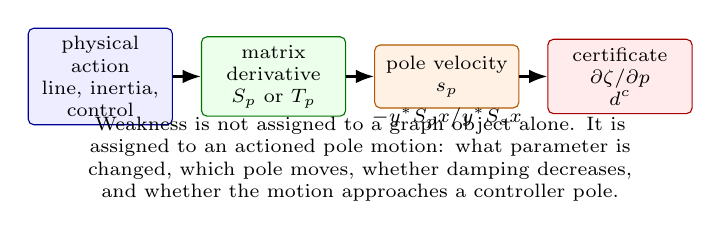
\begin{tikzpicture}[
  font=\scriptsize,
  >=Latex,
  box/.style={draw, rounded corners=2pt, align=center, inner sep=3pt, minimum height=8mm, text width=1.62cm},
  act/.style={box, fill=blue!7, draw=blue!60!black},
  der/.style={box, fill=green!8, draw=green!45!black},
  pole/.style={box, fill=orange!10, draw=orange!70!black},
  risk/.style={box, fill=red!8, draw=red!65!black},
  arr/.style={->, thick}
]
\node[act] (a) at (0,0) {physical action\\line, inertia, control};
\node[der] (b) at (2.2,0) {matrix derivative\\$S_p$ or $T_p$};
\node[pole] (c) at (4.4,0) {pole velocity\\$s_p$};
\node[risk] (d) at (6.6,0) {certificate\\$\partial\zeta/\partial p$\\$d^c$};
\draw[arr] (a) -- (b);
\draw[arr] (b) -- (c);
\draw[arr] (c) -- (d);
\node[align=center, text width=7.15cm, font=\scriptsize] at (3.3,-1.05)
{Weakness is not assigned to a graph object alone. It is assigned to an
actioned pole motion: what parameter is changed, which pole moves, whether
damping decreases, and whether the motion approaches a controller pole.};
\node[font=\scriptsize] at (4.4,-0.53)
{$-y^\ast S_px/y^\ast S_sx$};
\end{tikzpicture}
\caption{Local certificate pipeline. The graph enters through $S_p$ or $T_p$,
but the decision is made after the pole and damping-ratio derivatives are
computed.}
\label{fig:certificate_pipeline}
\end{figure}

The deliberately provocative engineering message is therefore narrow but sharp:
``more network'' is not the same statement as ``more damping,'' and ``high modal
visibility'' is not the same statement as ``best actuator.'' A reinforcement,
inertia change, or controller retuning must be judged by the pole it moves and
by the controller pole it moves toward or away from.

\section{Weak Elements Are Dynamic Certificates}

Let $p_e$ be an admissible strengthening action on a line $e$, and let $p_i$ be an admissible local action at bus $i$. Examples include increasing line admittance, adding damping, changing virtual inertia, or retuning a controller. For each action, define the local damping-margin derivative
\begin{equation}
  g_p(k)=\frac{\partial\zeta(s_k)}{\partial p}
  \label{eq:gp}
\end{equation}
for the pole family of interest. A positive $g_p$ means the action improves the damping ratio of that tracked pole; a negative value means the action damages it.

To distinguish ordinary damping-ratio geometry from control-resonant weakness, define the controller-pole distance and self-energy fraction
\begin{align}
  d_k^{c} &= \min_{\mu\in\spec(A_{cc})}
  \frac{|s_k-\mu|}{|s_k|+|\mu|+\epsilon},
  \label{eq:dist}\\
  \phi_k^{c} &=
  \frac{\left|y_k^\ast A_{ec}(s_kI-A_{cc})^{-2}A_{ce}x_k\right|}
  {\left|y_k^\ast S_s(s_k)x_k\right|+\epsilon}.
  \label{eq:phi}
\end{align}
Here $d_k^c$ measures proximity to condensed-control poles, while $\phi_k^c$ measures how much of the NEP denominator is supplied by the frequency-dependent control term.

\begin{definition}[Controller-aware weak link]
A line $e$ is weak for pole $s_k$ and action direction $p_e$ if
\begin{equation}
  g_{p_e}(k)<0 .
  \label{eq:weaklink}
\end{equation}
It is control-resonant weak if, additionally, $d_k^c$ decreases under the action and $\phi_k^c$ or the self-energy contribution dominates the retained-network terms in \eqref{eq:nepsens}.
\end{definition}

\begin{definition}[Controller-aware weak node]
A bus $i$ is weak for a pole family if at least one physically admissible local action $p_i$ gives $g_{p_i}(k)<0$, or if the bus strongly participates in a mode with high $\phi_k^c$ and small $d_k^c$. Thus a node is not weak in isolation; it is weak relative to a mode, an action, and a controller configuration.
\end{definition}

These definitions intentionally do not use graph centrality. The following proposition states why.

\begin{proposition}[Graph centrality cannot identify controller-aware weak elements]
Consider two linearized IBR grids with the same retained network graph and the same line centralities. Suppose $A_{ec}A_{ce}\neq0$ for a retained mode $s_k$. Then, by changing only the condensed controller block $A_{cc}$ and its residues while holding the graph fixed, the sign and magnitude of $\partial\zeta(s_k)/\partial p_e$ in \eqref{eq:zetasens} can change. Therefore no score that is a function only of the static graph can determine controller-aware weak links or weak nodes in general.
\end{proposition}

\begin{proof}
For fixed graph and fixed retained action derivative, expand the Schur self-energy around the condensed-control poles:
\begin{equation}
  A_{ec}(sI-A_{cc})^{-1}A_{ce}
  =
  \sum_j \frac{R_j}{s-\mu_j},
  \label{eq:residue}
\end{equation}
where $\mu_j\in\spec(A_{cc})$ and $R_j$ are residues determined by controller couplings. The pole sensitivity \eqref{eq:nepsens} contains both the self-energy numerator and the denominator derivative
\begin{equation}
  A_{ec}(sI-A_{cc})^{-2}A_{ce}
  =
  \sum_j \frac{R_j}{(s-\mu_j)^2}.
  \label{eq:residue2}
\end{equation}
Moving a controller pole $\mu_j$ near $s_k$, or changing the phase/sign of the associated residue through controller parameters, changes the complex direction of $s_p$. Through \eqref{eq:zetasens}, this can make $g_{p_e}(k)$ positive or negative while the graph, line centralities, and retained Laplacian are unchanged. Hence graph-only centrality cannot determine the weak-element sign.
\end{proof}

\begin{remark}
The proposition does not say that centrality is useless. It says that centrality is incomplete for IBR damping margins when controller poles and network modes interact. A central line may be harmless, and a non-central line may be dangerous, if the latter moves a retained mode toward a controller resonance.
\end{remark}

\subsection{Why Participation Is Not Enough}

Modal participation is closer to dynamics than graph centrality, but it is still not the complete weak-element object. A participation factor answers ``where does the current mode live?'' The planning question is different: ``what happens to the pole if I change this element?'' The second question requires the directional derivative \eqref{eq:nepsens}. For a line $e=(i,j)$, a static modal score may be based on $(q_i-q_j)^2$ or on power-flow loading. Such scores do not include $A_{cc}$, so they cannot see that the same line action can move a mode toward or away from a PLL pole. For a bus $i$, a large component of a critical eigenvector does not distinguish between adding damping, changing virtual inertia, retuning a PLL, or reinforcing adjacent branches. Those actions correspond to different $S_p(s)$ and may move the same pole in different directions.

Table~\ref{tab:baseline_objects} summarizes the distinction. The proposed certificate does not replace every score in the table; it identifies when a score is missing the dynamic mechanism needed for a damping-margin claim.

\begin{table}[t]
\caption{Weak-element objects and what they can certify.}
\label{tab:baseline_objects}
\centering
\scriptsize
\setlength{\tabcolsep}{2pt}
\begin{tabular}{p{0.27\columnwidth}p{0.28\columnwidth}p{0.30\columnwidth}}
\toprule
Object & Depends on & Missing for IBR damping\\
\midrule
Graph centrality & Static topology & Controller poles and action direction\\
Line loading & Operating flow & Pole movement and damping ratio\\
Modal participation & Current eigenvector & Directional action derivative\\
Frequency-only line score & $\partial|\Imag(s)|/\partial p$ & Decay-rate and self-energy terms\\
NEP weak certificate & $S_p,S_s,\spec(A_{cc})$ & Local; needs validation for finite actions\\
\bottomrule
\end{tabular}
\end{table}

\section{Control-Resonant Braess Mechanism}

Classical Braess effects concern network performance degradation after adding capacity. For damping margins, there are two different mechanisms that should not be conflated.

The first is geometric. Because $\zeta=-\Real(s)/|s|$, a line reinforcement can lower $\zeta$ if it raises oscillation frequency more than it improves decay. This can happen in scalar models and does not require controller resonance.

The second is controller-mediated. Let $p_e$ be line strengthening, and decompose the numerator of \eqref{eq:nepsens} into
\begin{equation}
  y^\ast S_{p_e}(s)x
  =
  A_e+B_e+C_e,
  \label{eq:abc}
\end{equation}
where $A_e$ is the retained stiffness/frequency contribution, $B_e$ is the retained-network residual or modal-rotation contribution, and $C_e$ is the condensed-control self-energy contribution. A strict control-resonant Braess certificate is
\begin{align}
  &\frac{\partial\zeta(s_k)}{\partial p_e}<0,
  \label{eq:cert1}\\
  &\frac{\partial d_k^c}{\partial p_e}<0,
  \label{eq:cert2}\\
  &|C_e|>\gamma\max(|A_e|,|B_e|),\quad C_e \text{ has damaging sign},
  \label{eq:cert3}
\end{align}
with the nearest condensed-control pole dominated by inverter/control states. In words, strengthening the line damages damping, pulls the network-family mode closer to a controller pole, and the self-energy term dominates the sensitivity. This is the Braess-like mechanism that is specific to controller-aware IBR dynamics.

\begin{proposition}[Control-resonant Braess certificate]
For a smooth tracked network-family pole $s_k(p_e)$, conditions \eqref{eq:cert1}--\eqref{eq:cert3} certify a controller-mediated reinforcement reversal. The reversal is not explained by static stiffness alone: if $|C_e|>\gamma\max(|A_e|,|B_e|)$ with $\gamma>1$, then the damaging first-order pole motion is dominated by the condensed-control self-energy.
\end{proposition}

\begin{proof}
Smoothness gives the first-order expansion
\[
  \zeta(s_k(p_e+\Delta p))=
  \zeta(s_k(p_e))+
  \frac{\partial\zeta}{\partial p_e}\Delta p+O(\Delta p^2).
\]
Condition \eqref{eq:cert1} makes the first-order change negative for small strengthening $\Delta p>0$. Condition \eqref{eq:cert2} states that the same action decreases the distance to the closest condensed-control pole, so the resolvent terms in \eqref{eq:residue}--\eqref{eq:residue2} grow rather than recede. Finally, \eqref{eq:cert3} rules out a retained-network explanation at first order, because the self-energy contribution is larger than both retained terms by factor $\gamma$ and has the damaging sign. Thus the observed local reversal is controller-resonant in the Schur-NEP sense.
\end{proof}

\subsection{Reproducible Audit Procedure}

The certificate is operationalized as follows. First, compute the full linearization and partition it as in \eqref{eq:partition}. Second, extract zeros of \eqref{eq:schur} by contour integration and match them to the full eigensolve only after extraction. Third, classify the pole family using the reconstructed condensed state
\[
  x_c(s_k)=(s_kI-A_{cc})^{-1}A_{ce}x_e(s_k),
\]
and the ratio
\[
  \pi_c(s_k)=
  \frac{\norm{x_c(s_k)}}{\norm{x_e(s_k)}+\norm{x_c(s_k)}} .
\]
Fourth, perturb a physical line parameter, rerun the power flow and eigensolve, and compare the finite-difference pole motion with \eqref{eq:nepsens}. Fifth, label a reversal resonant only if it satisfies \eqref{eq:cert1}--\eqref{eq:cert3} and the nearest condensed pole is controller dominated. This prevents ordinary frequency--damping tradeoffs from being mislabeled as a new Braess mechanism.

\section{Minimal Synthetic Witness}

Before moving to IEEE 39-bus, it is useful to see the mechanism in a system small
enough to inspect by hand. Consider the three-bus network in
Fig.~\ref{fig:synthetic}, with bus 1 used as the angle reference. The retained
angles are $\theta=[\theta_2,\theta_3]^T$, and the grounded Laplacian is
\begin{equation}
  L(w)=
  \begin{bmatrix}
  w_{12}+w_{23} & -w_{23}\\
  -w_{23} & w_{13}+w_{23}
  \end{bmatrix}.
  \label{eq:syntheticL}
\end{equation}
The retained network has $M=I$ and $D_0=d_0I$. A two-state controller is attached
through
\begin{align}
  \ddot\theta + d_0\dot\theta + L(w)\theta + Kz &=0,\\
  \dot z &= A_c z + B\dot\theta ,
  \label{eq:syntheticfull}
\end{align}
so that eliminating $z$ gives
\begin{equation}
  T(s)=s^2I+s\left[d_0I+K(sI-A_c)^{-1}B\right]+L(w).
  \label{eq:syntheticT}
\end{equation}
The numerical witness uses
\[
\begin{gathered}
w_{12}=0.8701,\quad w_{13}=3.6556,\quad w_{23}=3.9125,\\
d_0=0.7886,\qquad \spec(A_c)=-0.2216\pm j1.4783.
\end{gathered}
\]
The line action is a one-percent strengthening of the coupling line,
$w_{23}\leftarrow1.01w_{23}$.

A static synchronizing-stiffness screen sees only
\[
  \nu_{\max}(L):\quad 10.3284\rightarrow 10.4044,
\]
an increase of $0.74\%$. In that graph-only view, the network is simply
stronger. The full controller-aware pole tells the missing part:
\[
  s:\ -0.133247+j1.257268
  \rightarrow
  -0.133005+j1.258115,
\]
so
\[
  \zeta:\ 0.105391\rightarrow0.105132,
  \qquad
  \Delta\zeta=-2.59\times10^{-4}.
\]
At the same time, the distance from the tracked pole to the nearest controller
pole falls from $0.23804$ to $0.23734$. Thus the perturbation strengthens the
graph but moves the dynamic pole toward the controller resonance and reduces
damping.

\begin{figure}[t]
\centering
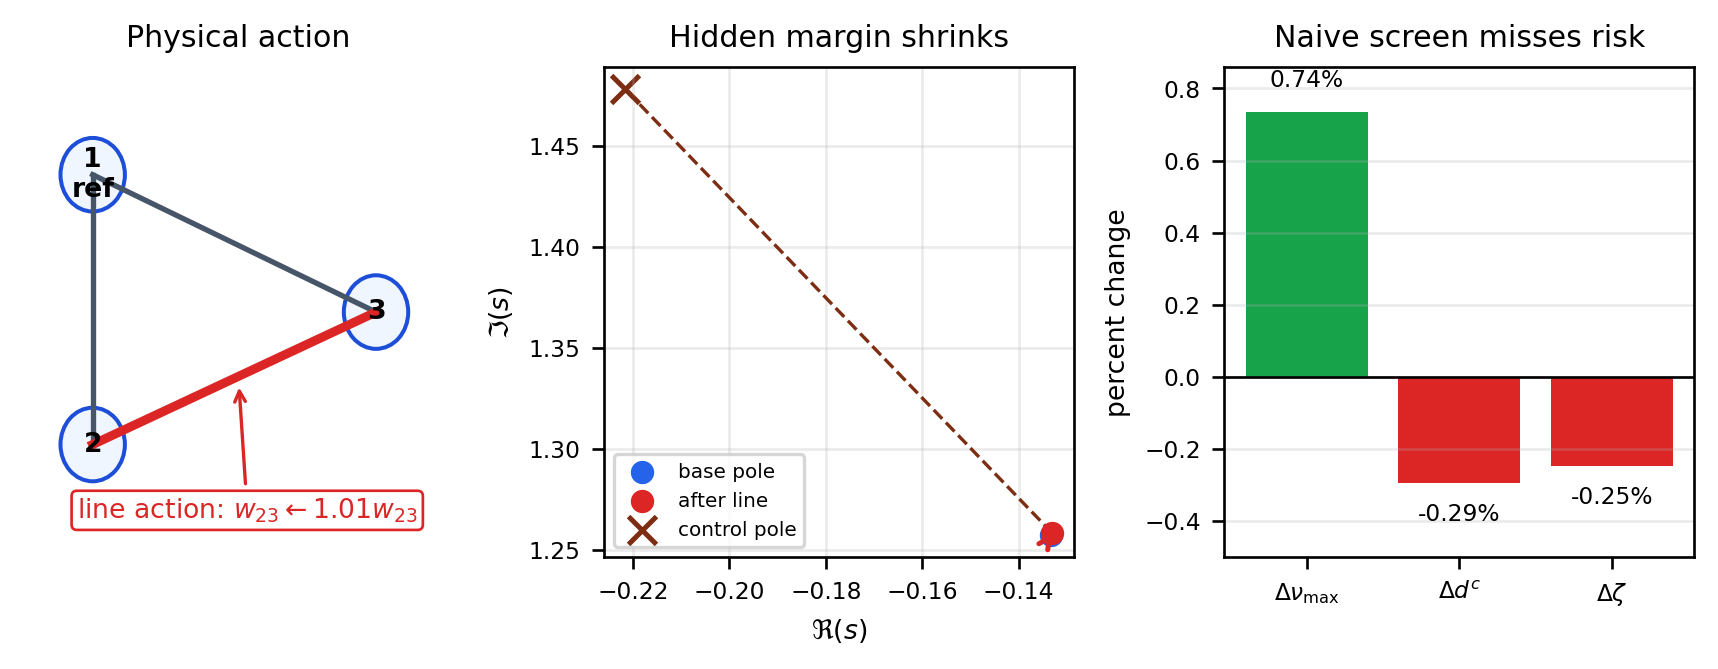
\includegraphics[width=\columnwidth]{figures/fig_synthetic_counterexample.png}
\caption{Minimal three-bus witness. Strengthening line 2--3 increases the
largest network stiffness, so a static synchronizing-torque screen sees a
stronger graph. The controller-aware pole, however, moves toward a control pole
and its damping ratio decreases.}
\label{fig:synthetic}
\end{figure}

This example is not presented as a realistic benchmark. It is a microscope for
the mechanism. It shows why the paper does not define weak links by edge
centrality or by stiffness increase alone. The relevant quantity is the pole
motion of the coupled network--controller object.

\section{IEEE 39-Bus ANDES Evidence}

The numerical evidence uses versioned ANDES IEEE 39-bus artifacts. The full ANDES eigensolve is the reference. The Schur NEP is solved by Beyn contour integration, not by fixed-point iteration. Zeros are extracted from contour moments and then locally polished by solving the intrinsic condition that the smallest singular value of $S_e(s)$ vanish; no ANDES target pole is supplied to the solver.

\begin{table}[t]
\caption{Controller-aware Schur-NEP bridge validation against full ANDES eigensolve.}
\label{tab:bridge}
\centering
\scriptsize
\begin{tabular}{lcccc}
\toprule
Case & Critical pole & Family & $\pi_c$ & Error\\
\midrule
no-PSS &
$-1.34635+j8.61104$ &
I & 0.680 &
$4.9{\times}10^{-14}\%$ f\\
base &
$-1.34601+j8.61148$ &
I & 0.653 &
$1.6{\times}10^{-13}\%$ f\\
Mix60 &
$-10.7514+j86.3419$ &
II & 0.853 &
$8.5{\times}10^{-11}\%$ f\\
\bottomrule
\end{tabular}
\vspace{1mm}

\raggedright
\footnotesize
The damping-ratio errors are $6.3{\times}10^{-13}\%$, $1.1{\times}10^{-12}\%$, and $2.5{\times}10^{-9}\%$, respectively. Mix60 is a 13.742 Hz PLL-family mode; its nearest condensed-control pole is $-10.5593+j86.246$ at distance $0.215$.
\end{table}

Table~\ref{tab:bridge} gives the bridge gate. In no-PSS and base cases, the critical poles are network-family modes. In Mix60, the damping-margin pole is a high-frequency control-family mode dominated by PLL states. This is the failure mode of scalar graph reductions: the critical object is not contained in a static Laplacian or nodal damping coefficient.

After the bridge passed, each tested line reinforcement reduced the physical ANDES branch $r$ and $x$ by $1/(1+\epsilon)$ with $\epsilon=0.01$, reran power flow, the full eigensolve, and the Schur-NEP contour solver. The audit covered Mix60, Mix60/no-PSS, and a soft-GFL negative-control profile. Table~\ref{tab:braess} summarizes the result.

\begin{table}[t]
\caption{Control-resonant line-reinforcement audit.}
\label{tab:braess}
\centering
\scriptsize
\setlength{\tabcolsep}{2pt}
\begin{tabular}{p{0.55\columnwidth}p{0.34\columnwidth}}
\toprule
Metric & Value\\
\midrule
Line/mode perturbations completed & 460\\
Global-margin reversals & 348\\
Network-family mode reversals & 232\\
Strict resonant records & 40\\
Median analytic-vs-NEP relative error & $8.08{\times}10^{-4}$\\
\midrule
Clearest case & Mix60/no-PSS, Line 20--34\\
Margin $\zeta$ & $0.123566\rightarrow0.123558$\\
Network-mode $\zeta$ & $0.133884\rightarrow0.133816$\\
Distance to matched $A_{cc}$ pole & $3.33227\rightarrow3.32790$\\
$A_e$ term & $-1.09{\times}10^{-9}$\\
$B_e$ term & $7.97{\times}10^{-9}$\\
$C_e$ term & $-6.87{\times}10^{-3}$\\
Control denominator fraction & 0.959\\
\bottomrule
\end{tabular}
\end{table}

\begin{figure}[t]
\centering
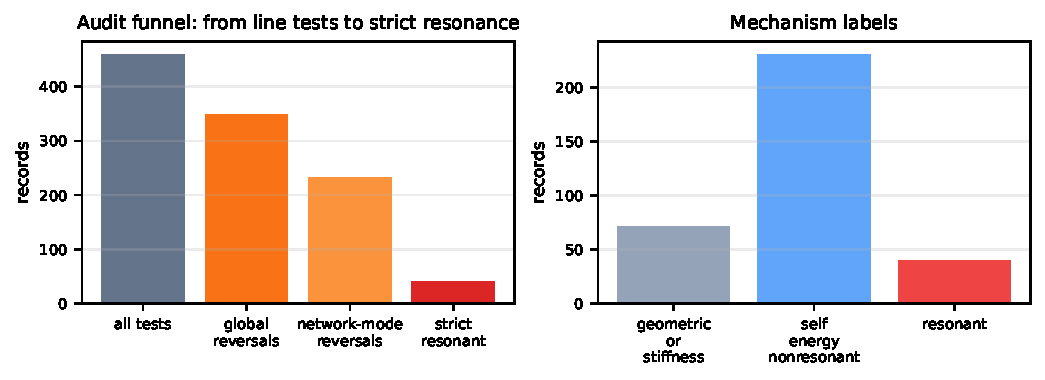
\includegraphics[width=\columnwidth]{figures/fig_audit_mechanism_summary.pdf}
\caption{Audit-level application view. Many line reinforcements reduce damping, but only a strict subset satisfies the controller-resonance certificate. This avoids confusing ordinary damping-ratio geometry with the proposed IBR-specific mechanism.}
\label{fig:audit_summary}
\end{figure}

The clearest case satisfies the strict certificate \eqref{eq:cert1}--\eqref{eq:cert3}. The damaging sensitivity is not a frequency-only effect: the retained stiffness term is negligible, while the condensed-control self-energy term sets the sign and magnitude. The finite-difference network-mode derivative is $-6.860{\times}10^{-3}$, and the analytic decomposition gives $-6.874{\times}10^{-3}$, a relative error of $2.0{\times}10^{-3}$. The nearest condensed pole is PLL-dominated, with leading states from PLL1 and inverter-control channels.

\begin{figure}[t]
\centering
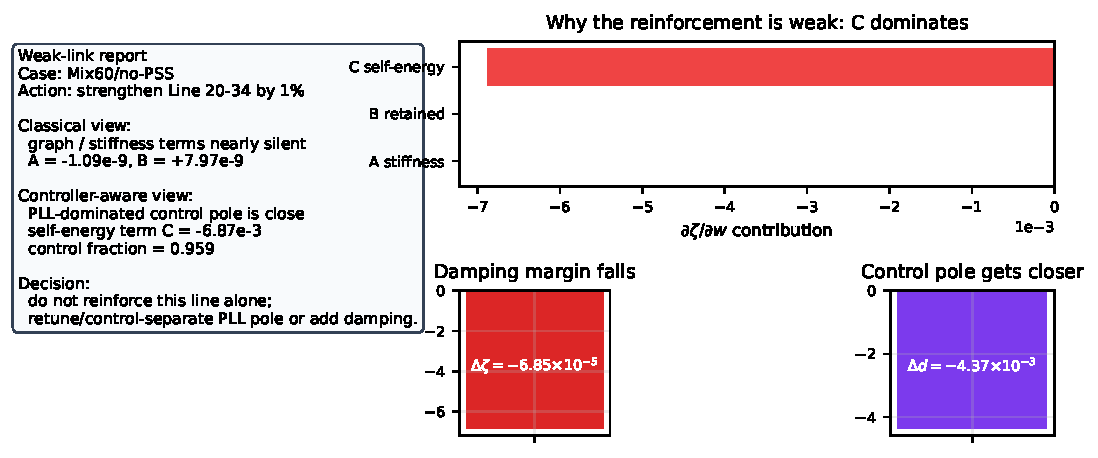
\includegraphics[width=\columnwidth]{figures/fig_application_weaklink_report.pdf}
\caption{Engineering report for the clearest weak link. A stiffness-only or graph-only view is nearly silent, but the controller-aware decomposition shows that the self-energy term dominates, the damping margin falls, and the mode moves closer to a PLL-dominated control pole.}
\label{fig:weaklink_report}
\end{figure}

The negative-control profile matters. Under the soft-GFL profile, the same spectral condition is removed: the network/control pole distance is much larger and the control-frequency denominator fraction falls. The audit therefore supports a mechanism claim, not a universal paradox claim. The resonant cases are modal-local and control-conditional; in these artifacts, the global margin is often still set by a control-family pole.

This is the practical failure mode the paper is meant to expose. A planner who sees only topology, loading, or retained stiffness would not flag Line 20--34 as a hidden damping-risk action in this operating point: the retained terms $A_e$ and $B_e$ are almost zero. The controller-aware certificate instead reports that the line action reduces damping because it decreases the separation between the network mode and a PLL-dominated pole. The recommended robustness action is therefore not ``add more copper on that branch'' by itself, but to retune or separate the implicated control pole, add damping, or choose a line action whose NEP sensitivity improves $\zeta$ without reducing $d_k^c$.

\subsection{What This Shows Against Static Rankings}

The ANDES evidence directly targets the title claim. The Mix60/no-PSS clearest case is not identified as weak because it is globally central in a graph-theoretic sense. It is identified as weak because the physical line-strengthening action has a negative NEP damping derivative and reduces the distance from a network-family pole to a PLL-dominated condensed-control pole. A graph-only score has no variable corresponding to the distance $d_k^c$ or the self-energy fraction $\phi_k^c$; therefore it cannot distinguish this line from a line with identical static graph role but different controller tuning.

The same logic applies to weak nodes. In an IBR grid, a bus may be a weak node for one intervention and not for another. If a local damping action moves the pole left, the bus is a useful damping-placement candidate. If a virtual-inertia or topology action rotates the pole toward a controller resonance, the same bus can be harmful for that action. The certificate therefore changes weak-node language from a scalar ranking to a typed statement:
\[
\text{bus } i \text{ is weak for mode } k
\text{ under action } p_i .
\]
This typed form is less convenient than centrality, but it is the form that remains meaningful when controller dynamics set the margin.

\subsection{Inertia Witness: Participation Can Pick the Wrong Machine}

The same warning appears for inertia placement. In the IEEE 39-bus base case, the
critical network-family pole has its largest state participation at
\texttt{GENROU\_1}: \texttt{omega GENROU 1} contributes $0.3682$ and
\texttt{delta GENROU 1} contributes $0.3422$. A common modal-participation
heuristic would therefore add inertia at that machine, located at bus 30.

The controller-aware NEP and the full ANDES eigensolve give the opposite
decision. Increasing the documented inertia parameter \texttt{GENROU.M} by one
percent at bus 30 reduces the damping margin. Increasing inertia at
\texttt{GENROU\_8}, bus 37, improves it. Table~\ref{tab:inertia_witness}
summarizes the witness.

\begin{table}[t]
\caption{IEEE 39-bus inertia witness: the most participating machine is not the best inertia action.}
\label{tab:inertia_witness}
\centering
\scriptsize
\setlength{\tabcolsep}{2pt}
\begin{tabular}{lcccc}
\toprule
Action & Bus & $M$ change & Post $\zeta_{\min}$ & $\Delta\zeta$\\
\midrule
Most participating \texttt{GENROU\_1} & 30 &
$8.400\!\rightarrow\!8.484$ &
0.153794 & $-6.36{\times}10^{-4}$\\
Best audited \texttt{GENROU\_8} & 37 &
$4.860\!\rightarrow\!4.9086$ &
0.154848 & $+4.18{\times}10^{-4}$\\
\bottomrule
\end{tabular}
\end{table}

The local NEP derivative predicts the damaging sign at bus 30:
$\partial\zeta/\partial\epsilon=-6.47\times10^{-2}$, while the full ANDES finite
difference gives $-6.36\times10^{-2}$. This is the cleanest weak-node message:
``where the mode lives'' and ``where an action improves damping'' are different
questions. The result should not be overextended. It is a documented
\texttt{GENROU.M} perturbation in full ANDES, not a claim about adding a new
generator with its own dispatch and controls, and not a validated GFM
virtual-inertia result.

\section{Rational-Filter Interpretation}

The same conclusion can be stated in graph-filter language. A polynomial graph filter $h(L)$ can reweight Laplacian modes, but it cannot create poles that are not in the graph operator. The Schur self-energy is different. In modal coordinates of the retained network, its entries are
\begin{equation}
  \widehat\Sigma_{ab}(s)=
  q_a^\ast A_{ec}(sI-A_{cc})^{-1}A_{ce}q_b ,
  \label{eq:modalself}
\end{equation}
so the filter depends on the evaluation point $s$ and on the condensed-control spectrum. Using the residue form \eqref{eq:residue},
\begin{equation}
  \widehat\Sigma_{ab}(s)=
  \sum_j \frac{q_a^\ast R_j q_b}{s-\mu_j}.
  \label{eq:rationalfilter}
\end{equation}
This is a rational filter over the network--controller interconnection, not a polynomial filter of the graph alone. It has two consequences.

First, weakness is mode-pair dependent. A line action may be benign for one network mode and harmful for another because the residues $q_a^\ast R_j q_b$ differ by mode pair. Second, weakness is frequency dependent. The same graph and the same line action can become dangerous only when the tracked pole lies near a controller pole. This explains why a static ranking can look reasonable in a synchronous-machine regime and fail in an IBR regime without any topological change.

The conference-level innovation is therefore not a new graph signal-processing algorithm. It is the identification of the correct signal path for damping-margin weakness:
\begin{equation}
\begin{aligned}
  \text{action}
  &\rightarrow S_p(s)
  \rightarrow \Delta s_k
  \rightarrow \Delta\zeta_k,\\
  &\hspace{4mm}(sI-A_{cc})^{-1}\ \text{retained.}
\end{aligned}
\label{eq:signalpath}
\end{equation}
Dropping the final resolvent collapses the problem back to graph centrality or modal participation and removes the mechanism observed in Table~\ref{tab:braess}.

\begin{table}[t]
\caption{Novelty boundary for the proposed conference paper.}
\label{tab:novelty}
\centering
\scriptsize
\setlength{\tabcolsep}{2pt}
\begin{tabular}{p{0.42\columnwidth}p{0.45\columnwidth}}
\toprule
Known ingredient & New use in this paper\\
\midrule
Schur complement and NEP sensitivity & Define weak elements as action-conditioned pole certificates\\
Graph/modal participation & Shown insufficient without controller-pole distance\\
Braess-style reversal language & Separated into geometric vs. control-resonant damping mechanisms\\
Beyn contour integration & Used as non-circular bridge validating the reduced object against ANDES\\
\bottomrule
\end{tabular}
\end{table}

\section{Discussion}

The proposed definitions shift weak-element analysis from graph ranking to mechanism attribution. A graph centrality score can say that a bus or line is structurally important, but it cannot say whether strengthening it increases damping, decreases damping by geometry, or decreases damping by pulling a network-family pole toward a PLL resonance. Those are different engineering problems. The first can be addressed by conventional reinforcement. The second requires damping-aware line ranking. The third may require controller retuning, pole separation, or avoiding a reinforcement that is attractive under static metrics.

\subsection{What This Gives to Power Engineers}

The practical output is a diagnostic workflow, not a decorative graph metric.
For each proposed action, the engineer obtains four quantities:
\begin{enumerate}
\item the tracked pole $s_k$ and its family, network-dominated or
controller-dominated;
\item the damping derivative $g_p=\partial\zeta(s_k)/\partial p$;
\item the controller-pole distance $d_k^c$ and whether the action shrinks it;
\item the dominant term in the sensitivity numerator, retained-network or
self-energy.
\end{enumerate}
Those four numbers answer a planning question that centrality cannot answer:
should the action be accepted, rejected, or replaced by a controller retuning?
In the Line 20--34 witness, the answer is not merely ``this line is weak.'' The
answer is: this line is weak for the tracked network-family mode under a
strengthening action because the action reduces damping and moves the mode
toward a PLL-dominated control pole. That statement is directly actionable:
avoid that reinforcement in that operating point, separate the implicated pole,
or choose an alternative line/control action whose certificate has the opposite
sign.

The controversial conclusions are deliberately stated with their scope:
\begin{itemize}
\item A stronger grid can be a weaker damping design if the added stiffness
pulls a mode toward a controller pole.
\item The most visible machine in a mode is not necessarily the best place to
add inertia; visibility is not a signed action derivative.
\item A stable IBR operating point can carry hidden margin debt: the pole is
stable, but already too close to controller dynamics for a static screen to be
trusted.
\end{itemize}
These are not universal laws. They are local, model-checked warnings. That is
precisely why the paper uses full eigensolve and Schur-NEP certificates rather
than a new centrality score.

The paper also clarifies what is not claimed. First, the NEP bridge is validated in three diagnostic IEEE 39-bus cases, not across all possible IBR dispatches. Second, the resonant Braess mechanism appears in a minority of strict line/mode records; it is not the dominant cause of every damping decrease. Third, the result is not a replacement for full ANDES eigensolve. It is a reduced diagnostic object that preserves the controller pole responsible for the mechanism.

For this conference-method contribution, this is the intended novelty boundary:
established tools such as Schur complements, contour NEP solvers, eigenvalue
sensitivities, and damping ratios are assembled into a controller-aware
definition of weak nodes and weak links. The new power-systems statement is
that IBR weak elements are action- and mode-conditioned dynamic certificates,
not graph-centrality objects.

\section{Conclusion}

Weak nodes and weak links in IBR grids should not be defined solely by static graph centrality. After controller states are condensed, the damping-margin problem is governed by a rational Schur NEP whose self-energy contains PLL and inverter-control poles. A local line or node action is weak when it moves a relevant pole in a damaging damping direction, especially when it also reduces the distance to a condensed-control pole. This framework explains a control-resonant Braess-like mechanism: line strengthening can reduce damping because it pulls a network-family mode toward a PLL-dominated controller pole. IEEE 39-bus ANDES artifacts validate the bridge and observe this mechanism under strict criteria.

The practical conclusion is uncomfortable but useful: a planning action that
looks robust in a graph can be a damping-risk action in the dynamics. More
copper, more inertia, or higher modal participation are not certificates of
stability. The certificate is the signed motion of the damping-margin pole. The
next step is not to invent another centrality score, but to benchmark these
certificates against conventional weak-node and weak-link rankings over broader
calibrated IBR operating ranges.

\begin{thebibliography}{99}

\bibitem{kundur1994power}
P. Kundur, \emph{Power System Stability and Control}. McGraw-Hill, 1994.

\bibitem{rogers2000oscillations}
G. Rogers, \emph{Power System Oscillations}. Kluwer Academic Publishers, 2000.

\bibitem{dorfler2014sync}
F. D\"orfler, M. Chertkov, and F. Bullo, ``Synchronization in complex networks of phase oscillators: A survey,'' \emph{Automatica}, vol. 50, no. 6, pp. 1539--1564, 2014.

\bibitem{braess1968}
D. Braess, ``\"Uber ein Paradoxon aus der Verkehrsplanung,'' \emph{Unternehmensforschung}, vol. 12, pp. 258--268, 1968.

\bibitem{tisseur2001}
F. Tisseur and K. Meerbergen, ``The quadratic eigenvalue problem,'' \emph{SIAM Review}, vol. 43, no. 2, pp. 235--286, 2001.

\bibitem{beyn2012}
W.-J. Beyn, ``An integral method for solving nonlinear eigenvalue problems,'' \emph{Linear Algebra and its Applications}, vol. 436, no. 10, pp. 3839--3863, 2012.

\bibitem{cui2021andes}
H. Cui, F. Li, and K. Tomsovic, ``Hybrid symbolic-numeric framework for power system modeling and analysis,'' \emph{IEEE Transactions on Power Systems}, vol. 36, no. 2, pp. 1373--1384, 2021.

\bibitem{andesdocs}
ANDES Developers, ``ANDES: Python software for symbolic-numeric power system simulation,'' 2026. [Online]. Available: \url{https://docs.andes.app/}

\bibitem{liyanage2025}
C. Liyanage \emph{et al.}, ``Strategic placement of grid-forming inverters considering spatiotemporal dynamics and composite stability index,'' \emph{IEEE Open Journal of the Industrial Electronics Society}, vol. 6, pp. 290--308, 2025.

\bibitem{setareh2025}
M. Setareh and M. S. Ghazizadeh, ``A systematic approach to compute power system oscillatory modes damping-ratio sensitivities considering different synchronous generator models,'' \emph{Computers and Electrical Engineering}, vol. 126, p. 110501, 2025.

\end{thebibliography}

\end{document}
